\section{Première modélisation abstraite}
	
%\subsection{}
%\paragraph{}
\subsection{Analyse}
   On veut initialement considérer très peu d'exigences. L'énoncé nous indique
   que seules les entrées et sorties de l'espace de l'aéroport sont étudiées. On effectue donc une étude formelle sur un système très simplifié où la piste et le tarmac ne sont pas différenciés. Nous étudions uniquement les échanges d'avions entre l'espace de l'aéroport et l'espace extérieur, ce qu'on modélise en utilisant deux events\footnote{un event est nommé transition dans la sémantique des machines à états finis. C'est un couple (garde/action). L'action s'exécute si la garde est vraie.}, decoller et atterrir :
   
   \begin{itemize}
   	\item extout lorsqu'un avion sort de l'espace extérieur pour rentrer dans l'espace aéroportuaire,
   	\item extin lorsqu'un avion entre dans l'espace extérieur.
   \end{itemize} 

\begin{figure}[H]
	\begin{center}	
		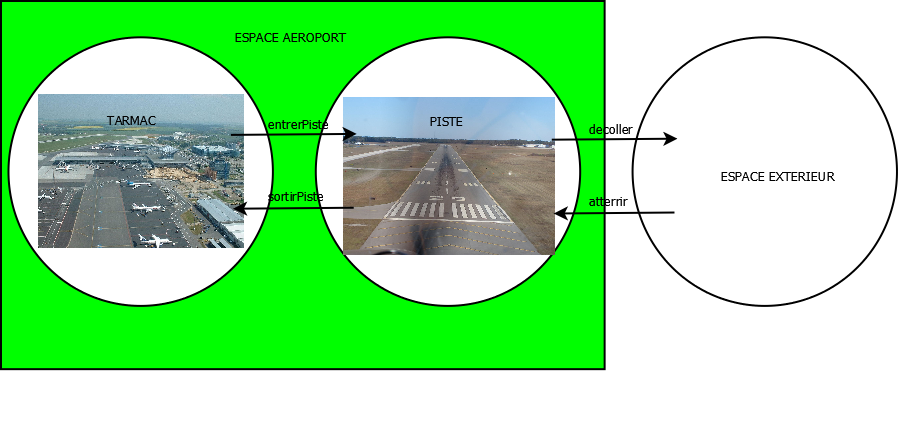
\includegraphics[scale=0.4]{images/0/mod0}
		\caption{Modèle abstrait : seuls les échanges avec l'extérieur sont pris en compte.}
		\label{mod0}
	\end{center}
\end{figure}


\subsection{Contexte du système}
L'état statique du système, nommé contexte dans la sémantique event-b, est caractérisé par ntmax, le nombre total maximum d'avions dans  l'espace de l'aéroport i.e. la capacité de l'aéroport, tarmac et piste confondues.
\begin{figure}[H]
	\begin{center}	
		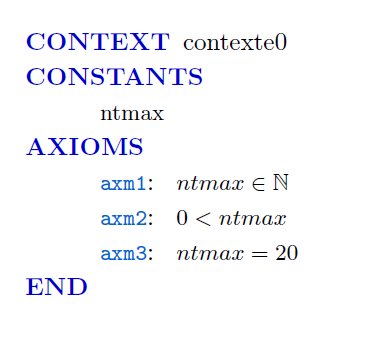
\includegraphics[scale=0.8]{images/0/ctx0}
		\caption{Etat statique du système}
		\label{ctx0}
	\end{center}
\end{figure}

\subsection{Machine :}

On fait abstraction de la piste. Ainsi, la seule variable à considérer est le nombre total d'avions présents dans l'espace de l'aéroport à un instant donné. On note nt cette variable. L'état dynamique du système, nommé machine dans la sémantique rodin/event-b, n'est constitué que de cette seule variable. Elle est respecte deux conditions ou \textit{invariants} :

\begin{figure}[H]
	\begin{center}	
		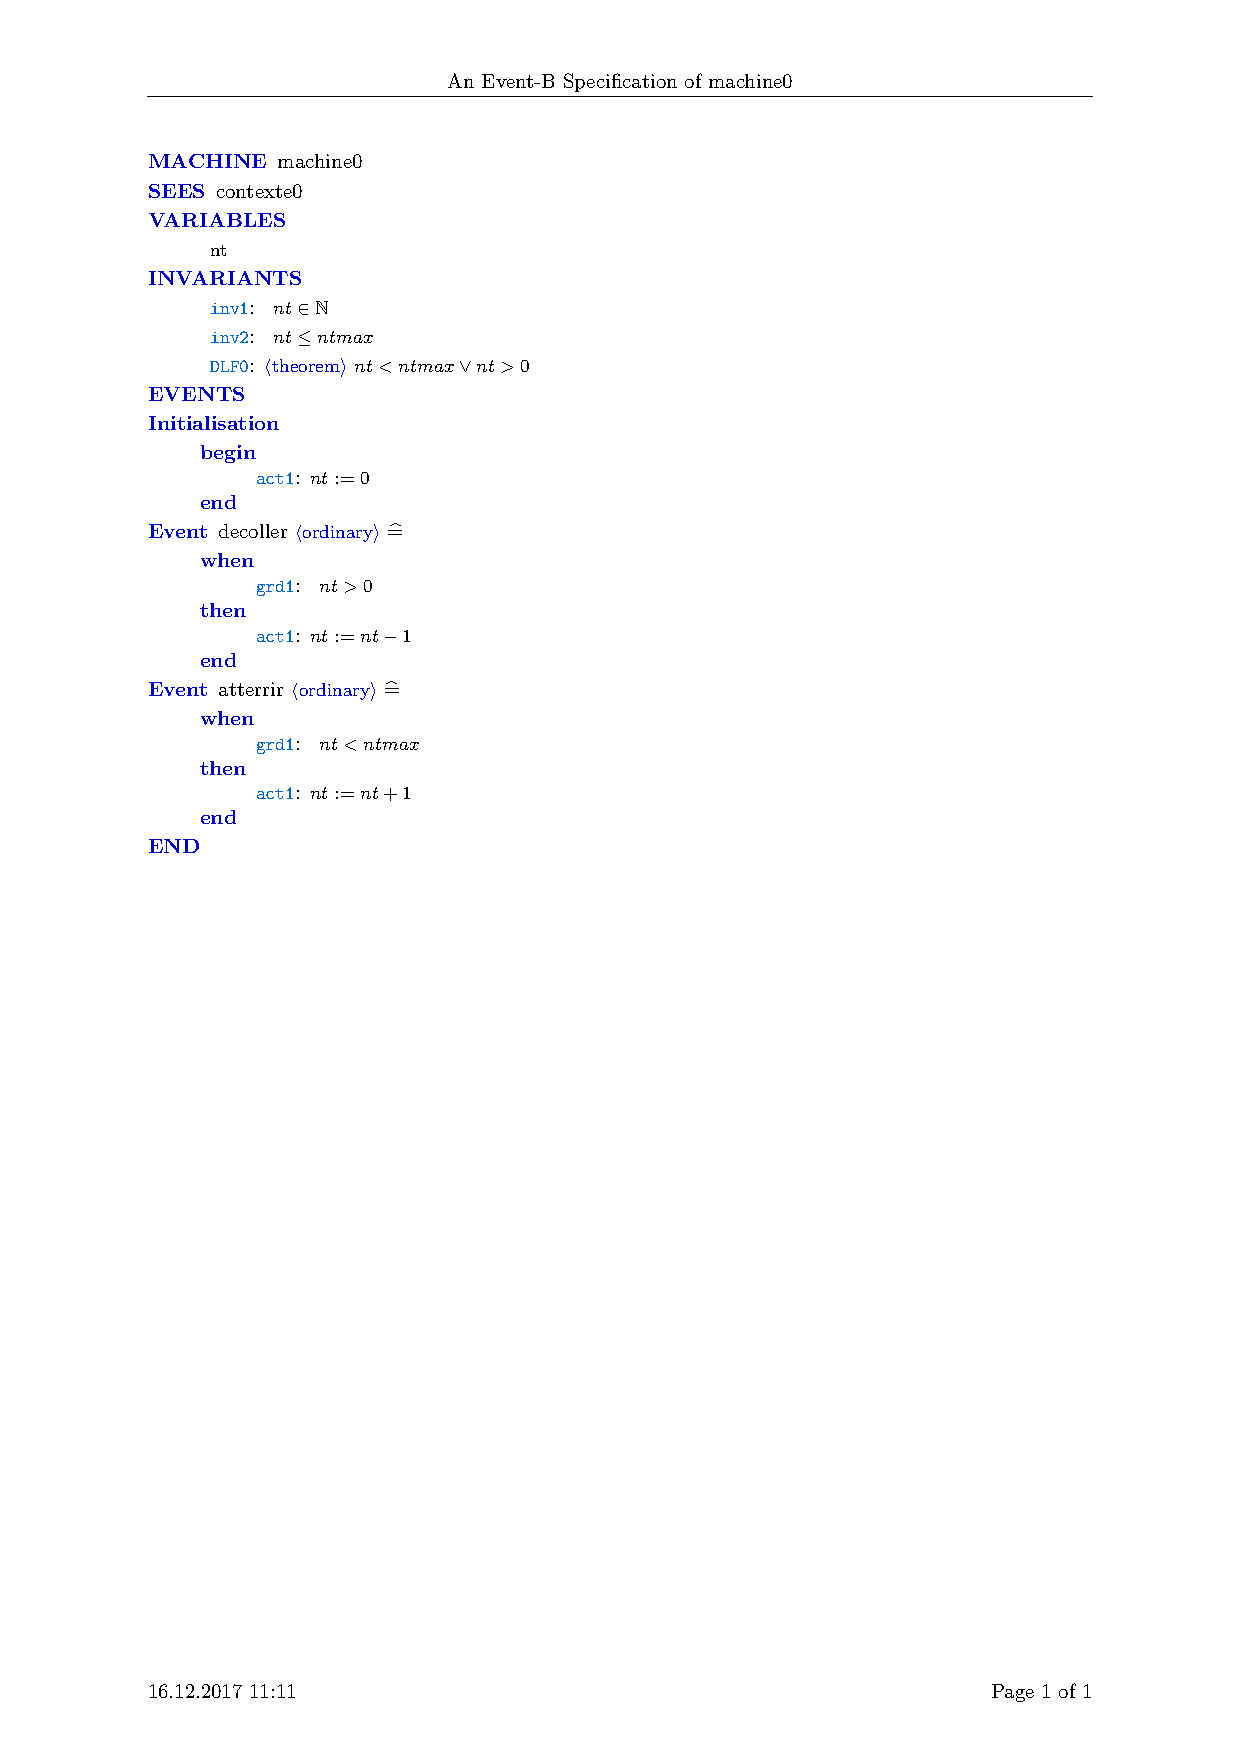
\includegraphics[scale=1]{images/0/machine0.png}
		\caption{Etat dynamique du système}
		\label{machine0}
	\end{center}
\end{figure}



\subsection{Preuves}
Pour débuguer le modèle formel initial, il a fallu ajouter deux gardes pour garantir un nombre d'avions compris entre 0 et 20 et éviter les deadlock.
Une preuve interactive, dans la perspective "proving", icône PP du "Proof control Panel", est nécessaire pour démontrer le thérorème d'invariant DLF0 pour prendre en compte toutes les hypothèses. C'est à ce stade que les règles d'inférences, en l'occurrence MON et OR\_L, mettent en évidence qu'un axiome supplémentaire est nécessaire qui impose ntmax > 0. Ici, on fixe ntmax = 20. En effet, si ntmax = 0, le système est bloqué dès l'origine. 

\begin{figure}[H]
	\begin{center}	
		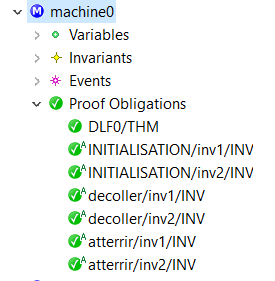
\includegraphics[scale=0.8]{images/0/proof0}
		\caption{Ajout de 2 gardes et d'un théorème pour éviter les blocages (invariant Deadlock free : DLF0)}
		\label{garde}
	\end{center}
\end{figure}

 Les exigences sont mises à jour pour tenir compte de ces oublis.

\begin{table} [H]
	
	\centering
	\rowcolors{2}{gray!65}{white}
	\begin{tabu}{|[2pt] p{1.7cm} | [2pt]p{15cm}|[2pt]}
		
		\tabucline[2pt]{-} \rowcolor{yellow}
		\Centering	\textbf{Label}& \Centering \textbf{Exigence}  \\ \tabucline[2pt]{-}
		
		\hline 
		FON-1&Le contrôleur doit autoriser les avions à décoller et atterrir  \\ 
		\hline 
		FON-1.1& \textcolor{red}{Le contrôleur doit fonctionner indéfiniment une fois lancé.}  \\ 
		\hline 
		FON-2	& Le nombre d'avions immobilisés sur le tarmac est limité à 20 y compris ceux en attente de décollage\textcolor{red}{ mais doit rester positif} \\ 
		\hline 
		FON-3& Des avions entrent sur et quittent la piste d'atterrissage décollage  \\ 
		\hline 
		FON-4& Des avions entrent sur le tarmac et le quittent  \\ 
		\hline 
		FON-5& La piste ne peut être occupée par un avion au décollage et un avion à l'atterrissage en même temps. \\ 
		\hline 
		FON-6& Le nombre de décollages ou atterrissages successifs n'est pas limité   \\ 
		\hline 
		FON-7& Le contrôleur doit fixer et délivrer les clearances à l'avance   \\ 
		\hline 
		FON-8& Le contrôleur ne doit autoriser l'avion qu'après l'envoi de son identifiant    \\ 
		\hline
		FON-9& Le contrôleur doit soit refuser, soit accepter, soit mettre en attente l'avion demandeur   \\ 
		\hline
		FON-10& Le contrôleur doit refuser la clearance après 10mn de mise en attente.   \\ 
		\hline 
		ENV-1 &Tout avion se dirigeant vers la piste doit avoir une autorisation de décoller \\ 
		\hline 
		ENV-2 &Le système est muni d'un capteur qui permet de compter les avions sur la piste \\ 
		\hline 
		ENV-3 &Le système est muni d'un capteur qui permet de compter les avions sur la tarmac \\ 
		\tabucline[2pt]{-}
	\end{tabu} 
	\caption{Tableau des exigences V2}
\end{table}
